\part{Complex systems}

\chapter{Computationally heavy}

\section{Introduction}

\section{Background}

Present here the combinatorial problems and the ways to solve them. 

\subsection{Langford problem}

C. Dudley Langford gave his name to a classic permutation problem ~\cite{Gard56, Simp83}.  
While observing his son manipulating blocks of different colors, he noticed that it was possible to arrange three pairs of different colored blocks (yellow, red, blue) in such a way that only one block separates the red pair - noted as pair 1 - , two blocks separate the blue pair - noted as pair 2 - and finally three blocks separate the yellow one - noted as pair 3 - , see Fig.~\ref{fig:lang}.
  
\begin{figure}[htbp]    
\begin{center}    
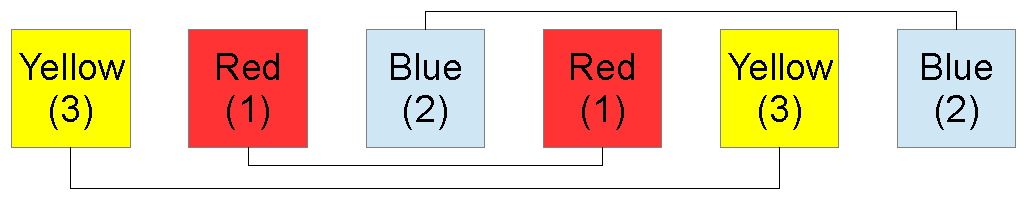
\includegraphics[scale=0.45]{figures/langford/lgf_cubes}   
\caption{L(2,3) arrangement} \label{fig:lang}    
\end{center}
\end{figure}
  
This problem has been generalized to any number $n$ of colors and any number $s$ of blocks having the same color. 
$L(s,n)$ consists in searching for the number of solutions to the Langford problem, up to a symmetry. % ... excepted symmetric ones. 
In November 1967, Martin Gardner presented $L(2,4)$ (two cubes and four colors) as being part of a collection of small mathematical games and he stated that $L(2,n)$ has solutions for all $n$ such that $n= 4k$ or $n = 4k-1$ ($k \in \mathbb{N} \setminus \{0\}$). 
The central resolution method consists in placing the pairs of cubes, one after the other, on the free places and backtracking if no place is available (see Fig.~\ref{backtrack} for detailed algorithm).

\begin{table}[t!]
\centering
\begin{tabular}{c r r r}
  \hline
  Instance & Solutions & Method & Computation time\\
  \hline
  \hline
  L(2,3) & 1 &  Miller algorithm & - \\
  L(2,4) & 1 & & - \\ 
  ... & ... & & ...  \\
  L(2,16) & 326,721,800 & & 120 hours  \\
  %\cline{1-3}
  L(2,19) & 256,814,891,280 & & 2.5 years (1999) DEC Alpha \\
  \hline
  \hline
  L(2,20) & 2,636,337,861,200 & Godfrey algorithm & 1 week \\
  %\cline{1-3}
  L(2,23) & 3,799,455,942,515,488 & &  4 days with CONFIIT \\
  %\cline{1-3}
  L(2,24) & 46,845,158,056,515,936 & & 3 months with CONFIIT \\
  L(2,27) & 111,683,611,098,764,903,232 & & - \\
  L(2,28) & 1,607,383,260,609,382,393,152 & & - \\
  \hline
\end{tabular}

\caption{Solutions and time with differents methods}
\label{tab:result_base}

\end{table}

The Langford problem has been approached in different ways: discrete mathematics results, specific algorithms, specific encoding, constraint satisfaction problem (CSP), inclusion-exclusion~\ldots~\cite{Mil00,apes-26,Smi00,larsen2009counting}.
In 2004, the last solved instance, $L(2,24)$, was computed by our team using a specific algorithm. (see Table \ref{tab:result_base}); $L(2,27)$ and $L(2,28)$ have just been computed but no details were given. 

The main efficient known algorithms are the following: the Miller backtrack method, the Godfrey algebraic method and the Larsen inclusion-exclusion method.
The Miller one is based on backtracking and can be modeled as a CSP; it allowed us to move the limit of explicits solutions building up to $L(2,21)$ but combinatorial explosion did not allow us to go further. 
Then, we use the Godfrey method to achieve $L(2,24)$ more quickly and then recompute $L(2,27)$ and $L(2,28)$, presently known as the last instances.
The Larsen method is based on inclusion-exclusion \cite{larsen2009counting}; although this method is effective, practically the Godfrey one is better. 
The lastest known work on the Langford Problem is a GPU implementation proposed in \cite{ASS_LGF} in 2015. Unfortunately this study does not provide any performance considerations but just gives the number of solution of $L(2,27)$ and $L(2,28)$.

\subsection{Miller algorithm}

In this part we present our multiGPU cluster implementation of the Miller's algorithm. First, we introduce the backtrack method. Then we present our implementation in order to fit the GPUs architecture. The last section presents our results. 

%\subsection{CSP and backtracking}

%Combinatorial problems are NP-complete\cite{GJ79} and can be described as a SATISFIABILITY problems (SAT) using a polynomial transformation. They can be transformed into CSP formalism.
%A Constraint Satisfaction Problem (CSP), first introduced by Montanari\cite{Mon74}, is defined as a triple $<X,D,C>$ where:
%$X=\{X_1,...,X_n\}$, a finite set of variables, $D=\{D_1,...,D_n\}$, their finite domains of values et $C=\{C_1,...,C_p\}$, a finite set of constraints.

%The goal in this formalism is to assign values in $D$ to $n$-uple $X$ respecting all the $C$ $p$-uple constraints.
%This approach is a large field of research. \cite{arbelaez2014gpu} developed \textit{local search} and compares GPU to CPU. 
%This first work brings to light that GPU is a real contributor to the global computation speed. \cite{campeotto2014exploring} proposes a solver using \textit{propagator} on a GPU architecture to solve CSP problems. 
%\cite{jenkins2011lessons} cares about GPU weak points, loading bandwidth and global memory latency.

%\subsection{CSP parallel resolution}
%\label{sec:CSP_resolution}

%Considering a basic approach, combinatorial problems formed into CSP can be represented as a tree search. Each level corresponds to a given variable, with values in its domain. Leaves of the tree correspond to a complete assignment (all variables are set). If it meets all the constraints this assignment is called an acceptor state. Depending on the constraints set, the satisfiability evaluation can be made either on complete or partial assignment.
%
%There are many ways to browse the tree and find the solutions: \emph{backtracking}, \emph{forward-checking}, \emph{backjumping}, etc. 
%We limit our method to the naive \emph{backtrack} resolution. We chose to evaluate the variables and their values in a static order; in a depth-first manner, the solution is built incrementally and if a partial assignment can be aborted, the branch is cut. A solution is found each time a leaf is reached.
%% presents a backtrack search with the previous CSP representation.
%
%The recommendation for performance on GPU accelerator is to use non test-based programs.
%Due to its irregularity, the basic \emph{backtracking} algorithm is suppose not to suit the GPU architecture.
%Thus a vectorized version is given when evaluating the assignments at the leaves' level, with one of the two following ways: assignments can be prepared on each tree node or totally set on final leaves before testing the satisfiability of the built solution, Fig.\ref{fig:algos}.
%
%\begin{figure}[htbf]
%\begin{minipage}[b]{0.45\linewidth}
%\begin{verbatim}
%for variable_1 
%   assignment
%   for variable_2
%      assignment
%      ...
%         for variable_n
%            assignment
%            test
%\end{verbatim}
%\end{minipage}
%\begin{minipage}[b]{0.45\linewidth}
%\begin{verbatim}
%for variable_1 
%   for variable_2
%   ...
%      for variable_n
%         assignments
%         test
%         
%         
%\end{verbatim}
%\end{minipage} 
%\caption{CSP regularized algorithms}
%\label{fig:algos}
%\end{figure} 
%
%With this method it is necessary to browse the entire tree but this requires using all the search space and it is too time-consuming.
%
%In order to overcome this we divide the work between CPU and GPU. The CPU generates some levels of the tree and creates tasks. Then GPU and CPU cores divide up the workload in order to achieve the generation on the latest levels of the tree. With this method, inconsistent branches can be cut on highest level and GPU/CPU cores only compute possibly consistent tasks.
%
%This representation enables a server-client model to distribute the tasks: the server generates independent sub-problems at a chosen depth in the tree, treated by clients. 
%Each client decomposes the sub-problem into tasks, distributed over the GPU/CPU cores, Fig.\ref{fig:parallel}.
%
%\begin{figure}[htbf]
%\centering 
%\includegraphics[scale=0.9]{figures/graphe_repartition}   
%\caption{Server client distribution} \label{fig:parallel}    
%\end{figure} 
%
%With this method numerous branches have been cut from the main tree during generation stage and GPU/CPU tasks are faster due to their lower depth. Despite the combinatorial explosion of this kind of problem, we can consider solving CSP in a massively parallel manner on multiGPU clusters.

\subsubsection{Backtrack resolution}

As presented above the Langford problem is known to be a highly irregular combinatorial problem. 
We first present here the general tree representation and the ways we regularize the computation for GPUs.
Then we show how to parallelize the resolution over a multiGPU cluster.

\paragraph{Langford's problem tree representation}
\label{sec:LGF_resolution}
In~\cite{HKS02}, we propose to formalize the Langford problem as a CSP  ({\it Constraint Satisfaction Problem}), first introduced by Montanari in \cite{Mon74}, and show that an efficient parallel resolution is possible. 
CSP formalized problems can be transformed into tree evaluations. %represented as trees. 
%The tree Here we intend to develop a specific algorithm taking into account the conclusion of our previous studies (memory management of memory and load balance) and transfer the tasks resolution into GPUs.\\
In order to solve $L(2,n)$, we consider the following tree of height $n$: see example of $L(2,3)$ in Fig.~\ref{fig:arbre}.

\begin{figure}[htb]
\centering
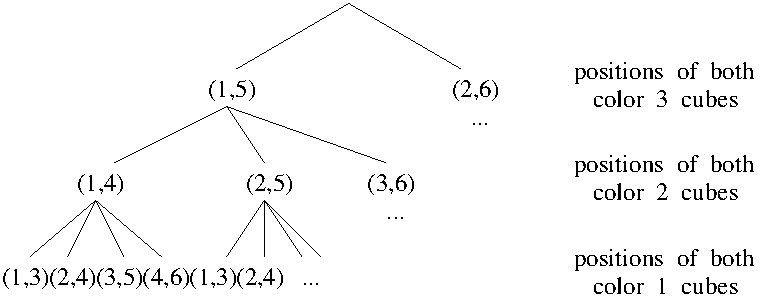
\includegraphics[scale=.65]{figures/langford/arbre_en}
\caption{Search tree for $L(2,3)$}
\label{fig:arbre}
\end{figure}


\begin{itemize}   
\item Every level of the tree corresponds to a color.
\item Each node of the tree corresponds to the placement of a pair of cubes without worrying about the other colors. Color $p$ is represented at depth $n-p+1$, where the first node corresponds to the first possible placement (positions 1 and $p+2$) and $i^{th}$ node corresponds to the placement of the first cube of color $p$ in position $i, \ i \in [1, \ 2n-1-p]$.
\item Solutions are leaves generated without any placement conflict.
\end{itemize}

There are many ways to browse the tree and find the solutions: \emph{backtracking}, \emph{forward-checking}, \emph{backjumping}, etc \cite{prosser93hybrid}. 
We limit our study to the naive \emph{backtrack} resolution and choose to evaluate the variables and their values in a static order; in a depth-first manner, the solutions are built incrementally and if a partial assignment can be aborted, the branch is cut. A solution is found each time a leaf is reached.
% presents a backtrack search with the previous CSP representation.

The recommendation for performance on GPU accelerators is to use non test-based programs.
Due to its irregularity, the basic \emph{backtracking} algorithm, presented on Fig.~\ref{backtrack}, is not supposed to suit the GPU architecture.
Thus a vectorized version is given when evaluating the assignments at the leaves' level, with one of the two following ways: assignments can be prepared on each tree node or totally set on final leaves before testing the satisfiability of the built solution (Fig.~\ref{regularized}).

\begin{figure}[htb]
\begin{minipage}[b]{0.45\linewidth}
\footnotesize
\begin{verbatim}
while not done do
 test pair            <- test
 if successful then 
   if max depth then
     count solution
     higher pair	                  
   else
     lower pair       <- remove
 else
   higher pair        <- add
\end{verbatim}
\caption{Backtrack algorithm}\label{backtrack}
\end{minipage}
\begin{minipage}[b]{0.45\linewidth}
\footnotesize
\begin{verbatim}
for pair 1 positions
  assignment                   <- add
  for pair 2 positions
    assignment                 <- add
    for ...
      for pair n positions
        assignment             <- add
        if final test ok then  
          count solution
\end{verbatim}
\caption{Regularized algorithm}\label{regularized}
\end{minipage}
\end{figure}

\paragraph{Data representation}

In order to count every Langford problem solution, we first identify all possible combinations for one color without worrying about the other ones. 
Each possible combination is coded within an interger, one bit to 1 corresponding to a cube presence, a 0 to its absence. This is what we called a \emph{mask}.
This way Fig.~\ref{fig:comb1} presents the possible combinations to place the one, two and three weight cubes for the $L(2,3)$ Langford instance.

Furthermore the masks can be used to evaluate the partial placements of a chosen set of colors: all the 1s correspond to occupied positions; the assignment is consistent \emph{iff} there are as many 1s as the number of cubes set for the assignment. 

With the aim to find solutions, we just have to go all over the tree and \emph{sum} one combination of each of the colors: a solution is found \emph{iff} all the bits of the sum are set to 1. 

Each route on the tree can be evaluated individually and independently; then it can be evaluated as a thread on the GPU.
This way the problem is massively parallel and can be, indeed, computed on GPU. Fig.~\ref{fig:pos_lgf} represents the tree masks' representation.

\begin{figure}[htb]
\begin{minipage}[b]{0.40\linewidth}
\centering
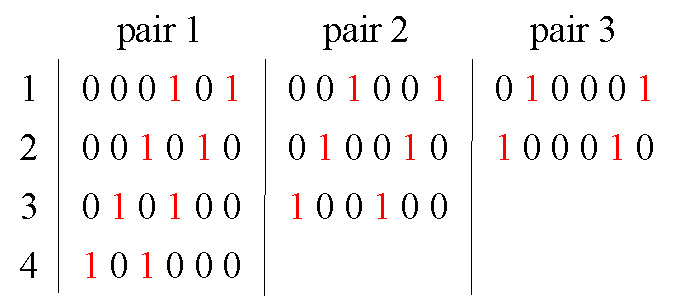
\includegraphics[width=\columnwidth]{figures/langford/positions_lgf}
\caption{ Bitwise representation of pairs positions in $L(2,3)$} \label{fig:comb1}
\end{minipage}
\hfill
\begin{minipage}[b]{0.55\linewidth}
\centering
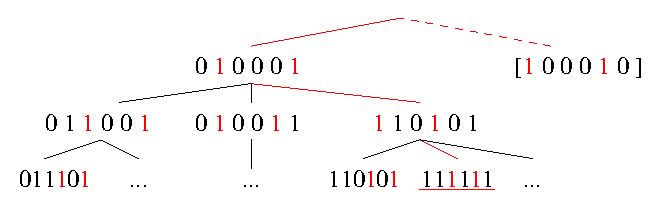
\includegraphics[width=\columnwidth]{figures/langford/pos_lgf_v2}
\caption{Bitwise representation of the Langford $L(2,3)$ placement tree}\label{fig:pos_lgf}
\end{minipage}
\end{figure}

\paragraph{Specific operations and algorithms}

Three main operations are required in order to perform the tree search. 
%The first one, allowing to check if a pair can be added to a given partial assignment, is only necessary for the original backtrack scheme.
%The second one, used for both backtrack and regularized methods, aims to add a pair to a given assignment. 
The first one, used for both backtrack and regularized methods, aims to add a pair to a given assignment. 
The second one, allowing to check if a pair can be added to a given partial assignment, is only necessary for the original backtrack scheme.
The last one is used for testing if a global assignment is an available solution: it is involved in the regularized version of the Miller algorithm.

\textbf{Add a pair -}
Top of Fig.~\ref{fig:test_et} presents the way to add a pair to a given assignment.
With a \emph{binary or}, the new mask contains the combination of the original mask and of the added pair.
This operation can be performed even if the position is not available for the pair (however the resulting mask is inconsistent). 

\textbf{Test a pair position -}
On the bottom part of the same figure, we test the positioning of a pair on a given mask. 
For this, it is necessary to perform a \emph{binary and} between the mask and the pair.
\begin{itemize}
	\item[] $=0$: \emph{success}, the pair can be placed here
	\item[] $\neq0$: \emph{error}, try another position
\end{itemize}

\textbf{Final validity test -}
The last operation is for \emph{a posteriori} checking. For example the mask $101111$, corresponding to a leaf of the tree, is inconsistent and should not be counted among the solutions.
The final placement mask corresponds to a solution \emph{iff} all the places are occupied, which can be tested as $\neg mask = 0$. % \rightarrow solution$ else $inconsistent$.
%We performed a \emph{binary not} on the mask. If there is a zero, so the mask is inconsistent, result will be different of zero. If the mask is full of $1$, result is zero, so we can add one to the number of solutions.
\\

Using this data representation, 
we implemented both \emph{backtrack} and \emph{regularized} versions of the Miller algorithm, as presented in Fig.~\ref{backtrack} and \ref{regularized}.
% C'est là que je veux changer la structure ....
%: the original backtrack for CPU computation and the regularized one for GPUs.
%As we have seen above, the regularized algorithm is unsuitable due to combinatorial explosion, that is why we use the hybrid method on a distributed architecture.
\\
The next section presents the way we hybridize these two schemes in order to get an efficient parallel implementation of the Miller algorithm.

%%%%%%%%%%%%%%%%%%%%%%%%%%%%%%%%%%%%%%%%
\paragraph{Hybrid parallel implementation}
\label{section:parallel_backtrack}
This part presents our methodology to implement Miller's method on a multiGPU cluster.

\textbf{Tasks generation -}
In order to parallelize the resolution we have to generate tasks. 
Considering the tree representation, we construct tasks by fixing the different values of a first set of variables [pairs] up to a given level. Choosing the development level allows to generate as many tasks as necessary. This leads to a \textit{Finite number of Irregular and Independent Tasks} (\emph{FIIT} applications \cite{krajecki1999object}). 

\textbf{Cluster parallelization -} 
The generated tasks are independent and we spread them in a client-server manner: a server generates them and makes them available for clients. As we consider the cluster as a set of CPU-GPU(s) machines, the clients are these machines. 
At the machines level, the role of the CPU is, first, to generate work for the GPU(s): it has to generate sub-tasks, by continuing the tree development as if it were a second-level server, and the GPU(s) can be considered as second-level client(s). \\
The sub-tasks generation, at the CPU level, can be made in parallel by the CPU cores. Depending on the GPUs number and their computation power the sub-tasks generation rhythm may be adapted, to maintain a regular workload both for the CPU cores and GPU threads: some CPU cores, not involved in the sub-tasks generation, could be made available for sub-tasks computing.\\
This leads to the 3-level parallelism scheme presented in Fig.~\ref{fig:parallel}, where $p$, $q$ and $r$ respectively correspond to: ($p$) the server-level tasks generation depth, ($q$) the client-level sub-tasks generation one, ($r$) the remaining depth in the tree evaluation, \textit{i.e.} the number of remaining variables to be set before reaching the leaves.  

\textbf{\emph{Backtrack} and \emph{regularized} methods hybridization -} 
The Backtrack version of the Miller algorithm suits CPU execution and allows to cut branches during the tree evaluation, reducing the search space and limiting the combinatorial explosion effects. A regularized version had to be developed, since GPUs execution requires synchronous execution of the threads, with as few branching divergence as possible; however this method imposes to browse the entire search space and is too time-consuming. \\
We propose to hybridize the two methods in order to take advantage of both of them for the multiGPU parallel execution: 
for tasks and sub-tasks generated at sever and client levels, the tree development by the CPU cores is made using the backtrack method, cutting branches as soon as possible [and generating only possible tasks]; when computing the sub-tasks generated at client-level, the CPU cores involved in the sub-tasks resolution use the backtrack method and the GPU threads the regularized one. 

%With this method it is necessary to browse the entire tree but this requires using all the search space and it is too time-consuming.

%In order to overcome this we divide the work between CPU and GPU. The CPU generates some levels of the tree and creates tasks. Then GPU and CPU cores divide up the workload in order to achieve the generation on the latest levels of the tree. 
%With this method, inconsistent branches can be cut on highest level and GPU/CPU cores only compute possibly consistent tasks.

%This representation enables a server-client model to distribute the tasks: the server generates independent sub-problems at a chosen depth in the tree, treated by clients. 
%Each client decomposes the sub-problem into tasks, distributed over the GPU/CPU cores, Fig.~\ref{fig:parallel}.

\begin{figure}[t!]
\begin{minipage}[b]{0.5\linewidth}
\centering
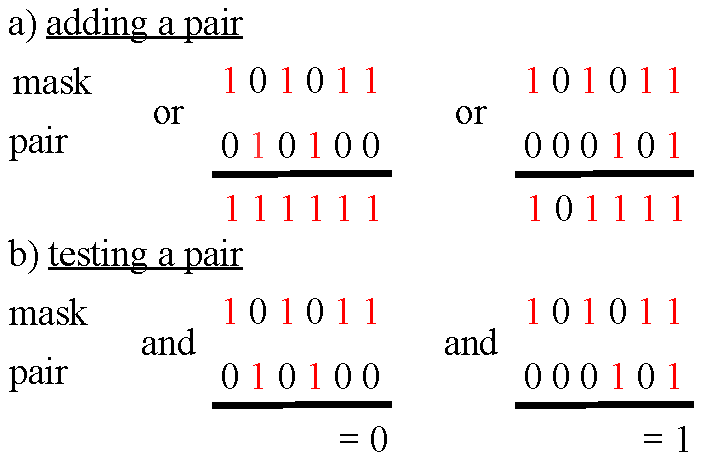
\includegraphics[scale=.5]{figures/langford/test_gen}
\caption{Testing and adding position} \label{fig:test_et}
\end{minipage}
\begin{minipage}[b]{0.5\linewidth}
\centering 
\includegraphics[scale=.75]{figures/langford/graphe_repartition}   
\caption{Server client distribution} \label{fig:parallel} 

\end{minipage}
\end{figure}

%By doing so numerous branches have been cut from the main tree during generation stage and GPU/CPU tasks are faster due to their lower depth. Despite the combinatorial explosion of this kind of problem, we can consider solve it in a massively parallel manner on multiGPU clusters.
 
%The tree representation allows to generate tasks at a chosen level, which leads to a \textit{Finite number of Irregular and Independent Tasks} (\emph{FIIT} applications \cite{krajecki1999object}).
%We set up a server-client distribution. The server, client and GPU parts have their own development depth, respectively $p$, $q$ and $r$, $p+q+r=n$, Fig.~\ref{fig:parallel}.
%\begin{itemize}
%\item \texttt{Server} generates sub-problems by placing $p$ pairs on masks with the $backtrack$ algorithm.
%\item \texttt{Client} starts with a mask generated by the server and produces tasks by adding $q$ pairs in the initial mask, with the $backtrack$ algorithm. Then the client creates specific tasks by pre-computing the available positions for placing pairs. For example with the $10100110$ mask the second pair can be placed on only two positions, $01001000$ and $00001001$, that match positions 2-5 and 5-8. Instead of browsing all the 5 positions and test, the GPU just has to try 2 positions for this pair. Thus we greatly reduce the GPU load computation.
%\item \texttt{CPUs and GPUs} can compute in competition. Whereas CPUs use standard backtrack, GPUs generate leaves using the regularized method and adding successive pairs on their masks without any test.  
%\end{itemize}

\subsubsection{Experiments tuning}

In order to take advantage of all the computing power of the GPU we have to refine the way we use them: this section presents the experimental study required to choose optimal settings. This tuning allowed us to prove our proposal on significant instances of the Langford problem.

\paragraph{Registers, blocks and grid}

In order to use all GPUs capabilities, the first way was to fill the blocks and grid. To maximize occupancy (ratio between active warps and the total number of warps) NVIDIA suggests to use 1024 threads per block to improve GPU performances and proposes a CUDA occupancy calculator\footnote{\url{http://developer.download.nvidia.com/compute/cuda/CUDA_Occupancy_calculator.xls}}. But, confirmed by the Volkov's results\cite{Volkov}, we experimented that better performances may be obtained using lower occupancy. Indeed, another critical criterion is the inner GPU registers occupation. 
The optimal number of registers ($57$ registers) is obtained by setting 9 pairs placed on the client for $L(2,15)$, thus 6 pairs are remaining for GPU computation.

\begin{figure}[t!]
\centering
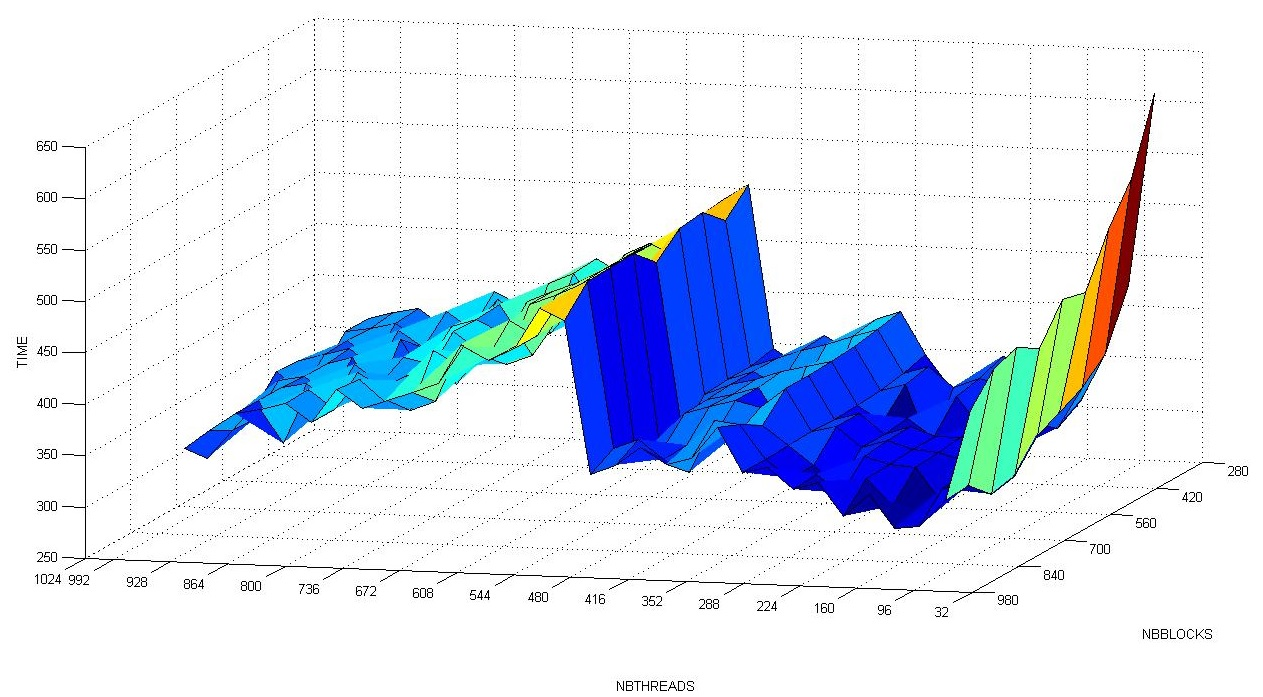
\includegraphics[scale=.4]{figures/langford/graphe_15_9}
\caption{Time depending on grid and block size on $n=15$}
\label{f7}
\end{figure}

In order to tune the blocks and grid sizes, we performed tests on the ROMEO architecture. 
%0 With this value we obtained an optimized number of registers by thread . 
Fig.~\ref{f7} represents the time in relation with the number of blocks per grid and the number of threads per block. The most relevant result, observed as a local minimum on the 3D surface, is obtained near 64 or 96 threads per block; for the grid size, the limitation is relative to the GPU global memory size.
It can be noted that we do not need shared memory because their are no data exchanges between threads. This allows us to use the total available memory for the L1 cache for each thread.

\paragraph{Streams}

%\subsubsection{Overlap CPU/GPU}

A client has to prepare work for GPU. There are four main steps: generate the tasks, load them into the device memory, process the task on the GPU and then get the results.

CPU-GPU memory transfers cause huge time penalties (about 400 cycles latency for transfers between CPU memory and GPU \emph{device memory}). 
At first, we had no overlapping between memory transfer and kernel computation because the tasks generation on CPU was too long compared to the kernel computation.
To reduce the tasks generation time we used OpenMP in order to use the eight available CPU cores.
Thus CPU computation was totally hidden by memory transfers and GPU kernel computation. We tried using up to 7 streams; as shown by Fig.~\ref{fig:streams}, using only two simultaneous streams did not improve efficiency because the four steps did not overlap completely; the best performances were obtained with three streams; the slow increase in the next values is caused by synchronization overhead and CUDA streams management.




\begin{figure}[htb]
\begin{minipage}[b]{0.48\linewidth}
\centering
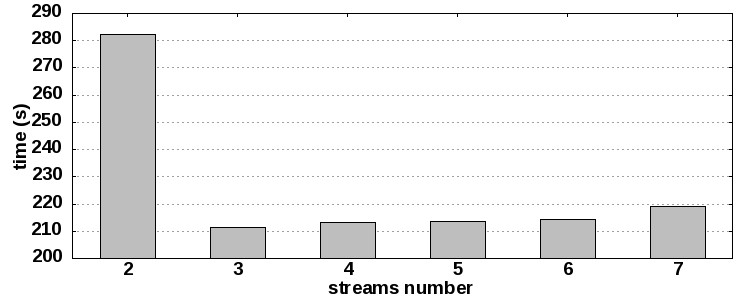
\includegraphics[width=\columnwidth]{figures/langford/streams.jpeg}
\caption{Computing time depending on streams number}
\label{fig:streams}
\end{minipage}
\hfill
\begin{minipage}[b]{0.48\linewidth}
\centering
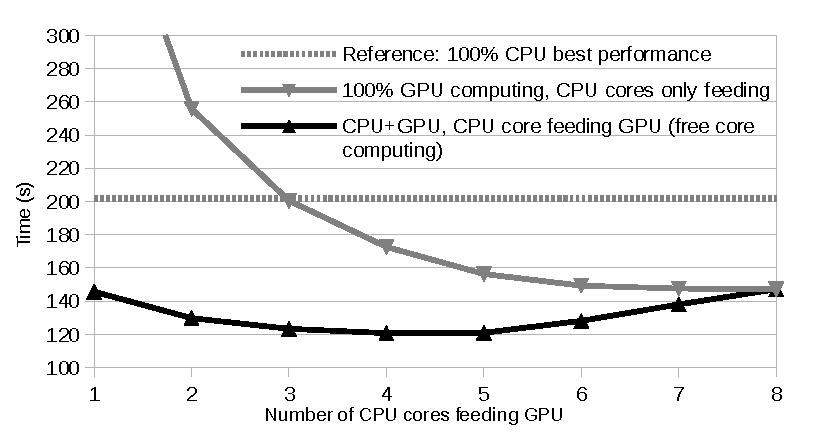
\includegraphics[width=\columnwidth]{figures/langford/graphe_cores.pdf}
\caption{CPU cores optimal distribution for GPU feeding}\label{cores_rep}
\end{minipage}
\end{figure}

\paragraph{Setting up the server, client and GPU depths}
We now have to set the depths of each actor, server $(p)$, client $(q)$ and GPU $(r)$ (see Fig.~\ref{fig:parallel}).

First we set the $r = 5$ for large instances because of the GPU limitation in terms of registers by threads, exacerbated by the use of numerous $64bits$ integers. For $r \geq 6$, we get too many registers (64) and for $r \leq 4$ the GPU computation is too fast compared to the memory load overhead.

Clients are the buffers between the server and the GPUs: 
$q = n - p- r$.
So we have conducted tests by varying the server depth, $p$. The best result is obtained for $p=3$ and performance decreases quickly for higher values. This can be explained since more levels on the server generates smaller tasks; thus GPU use is not long enough to overlap memory exchanges.
% because with more levels on the server, tasks are smaller and then the GPU work is not long enough in view of memory exchanges.

\paragraph{CPU: Feed the GPUs and compute}
The first work of CPU cores is to prepare tasks for GPU so that we can generate overlapping between memory load and kernel computation. In this configuration using eight cores to generate GPU tasks under-uses CPU computation power. It is the reason why we propose to use some of the CPU cores to take part of the sub-problems treatment. Fig.~\ref{cores_rep} represents computation time in relation with different task distributions between CPU and GPU.
We experimentally demonstrated that only 4 or 5 CPU cores are enough to feed GPU, the other ones can be used to perform backtrack resolution in competition with GPUs.

\subsubsection{Results}

\paragraph{Regularized method results}
We now can show the results obtained for our massively parallel scheme using the previous optimizations, comparing the computation times of successive instances of the Langford problem. These tests were performed on 20 nodes of the ROMEO supercomputer, hence 40 CPU/GPU machines.

The previous limit with Miller's algorithm was $L(2,19)$, obtained in 1999 after 2.5 years of sequential effort and at the same time after 2 months with a distributed approach\cite{Mil00}. Our computation scheme allowed us to obtain it in less than 4 hours (Table \ref{tab:result_base_regu}), this being not only due to Moore law progress.\\
Note that the computation is 1.6 faster with CPU+GPU together than using 8 CPU cores. In addition, the GPUs compute $200000\times$ more nodes of the search tree than the CPUs, with a faster time.

\begin{table}[htb]
\begin{minipage}[b]{0.5\linewidth}

\centering
\begin{tabular}{l r r r}
					\hline
					$n$ & CPU (8c) &  GPU (4c) +  &  \hspace*{-.8em}CPU (4c) \\
					\hline
					\hline
					15	& 2.5 & 1.5 & \\
					16  & 21.2 &14.3 & \\
					17  & 200.3 &120.5 &\\
					18  & 1971.0 &1178.2 &\\
					19  & 22594.2 & 13960.8 & \\ 
					\hline
\end{tabular}
					
\caption{Regularized method (seconds)}

\label{tab:result_base_regu}

\end{minipage}
\begin{minipage}[b]{0.5\linewidth}

\centering
\begin{tabular}{ l r r r }
					\hline
					$n$ & CPU (8c) &  GPU (4c) +  &  \hspace*{-.8em}CPU (4c) \\
					\hline
					\hline
					17  & 29.8 & 7.3&\\
					18  & 290.0 & 73.6&\\
					19  & 3197.5 & 803.5& \\
					20  & -- & 9436.9 &\\
					21  & -- & 118512.4& \\ 
					\hline
\end{tabular}
					
\caption{Backtrack  (seconds)}
\label{tab:result_backtrack}

\end{minipage}
\end{table}

The computation time between two different consecutive instances being multiplied by $10$ approximately, this could allow us to obtain $L(2,20)$ in a reasonable time.


\paragraph{Backtracking on GPUs}

It appears at first sight that using backtracking on GPUs without any regularization is a bad idea due to threads synchronization issues.
But in order to compare CPU and GPU computation power in the same conditions we decide to implement the original backtrack method on GPU (see Fig.~\ref{backtrack}) with only minor modifications.
In these conditions we observe very efficient work of the NVIDIA scheduler, which perfectly handles threads desynchronization.
Thus we use the same server-client distribution as in \ref{section:parallel_backtrack}, each client generates masks for both CPU and GPU cores. 
The workload is then statically distributed on GPU and CPU cores.
Executing the backtrack algorithm on a randomly chosen set of sub-problems allowed us to set the GPU/CPU distribution ratio experimentally to 80/20\%, 

The experiments were performed on 129 nodes of the ROMEO supercomputer, hence 258 CPU/GPU machines and one node for the server. 
Table \ref{tab:result_backtrack} shows the results with this configuration. 
This method first allowed us to perform the computation of $L(2,19)$ in less than 15 minutes, $15\times$ faster than with the regularized method; then, we pushed the limitations of the Miller algorithm up to $L(2,20)$ in less than 3 hours and even $L(2,21)$ in about $33$ hours\footnote{Even if this instance has no interest since it is known to have no solution}.

This exhibits the ability of the GPU scheduler to manage highly irregular tasks. It proves that GPUs are adapted even to solve combinatorial problems, which they were not supposed to be.

\subsection{Godfrey's algebraic method}
The previous part presents the Miller algorithm for the Langford problem, this method cannot achieve bigger instances than the $L(2,21)$.\\
An algebraic representation of the Langford problem has been proposed by M. Godfrey in 2002.
In order to break the limitation of $L(2,24)$ we already used this very efficient problem specific method.
In this part we describe this algorithm and optimizations, and then our implementation on multiGPU clusters.
\subsubsection{Method description}
Consider $L(2,3)$ and $X=(X_1,X_2,X_3,X_4,X_5,X_6)$. 
It proposes to modelize $L(2,3)$ by 
$F(X,3) = (X_1X_3+X_2X_4+X_3X_5+X_4X_6)\times (X_1X_4+X_2X_5+X_3X_6)\times (X_1X_5+X_2X_6) $

In this approach each term represents a position of both cubes of a given color and a solution to the problem corresponds to a term developed as $(X_1X_2X_3X_4X_5X_6)$; thus the number of solutions is equal to the coefficient of this monomial in the development. More generally, the solutions to $L(2,n)$ can be deduced from $(X_1X_2X_3X_4X_5...X_{2n})$ terms in the development of $F(X,n)$.

If \ \ $G(X,n) = X_1 ... X_{2n} F(X,n)$ then it has been shown that: 


$\sum\limits_{(x_1,...,x_{2n}) \in \{-1,1\}^{2n}} G(X,n)_{(x_1,...,x_{2n})} =  2^{2n+1}L(2,n)$

So \hspace*{2cm}
$\sum\limits_{(x_1,...,x_{2n}) \in \{-1,1\}^{2n}} \big( \prod\limits_{i=1}^{2n} x_i \big) \prod\limits_{i=1}^{n} \sum\limits_{k=1}^{2n-i-1} x_kx_{k+i+1} = 2^{2n+1} L(2,n)$
\\

\noindent That allows to get $L(2,n)$ from polynomial evaluations.
The computational complexity of $L(2,n)$ is of $O(4^n\times n^2)$ and an efficient big integer arithmetic is necessary. This principle can be optimized by taking into account the symmetries of the problem and using the Gray code: these optimizations are described below.

\subsubsection{Optimizations}
Some works focused on finding optimizations for this arithmetic method\cite{CReSTIC-1154}. Here we explain the symmetric and computation optimizations used in our algorithm.

\paragraph{Evaluation parity}
As $[F(-X,n) = F(X,n)]$, $G$ is not affected by a global sign change. 
In the same way the global sign does not change if we change the sign of each pair or impair variable.

Using these optimizations we can set the value of two variables and accordingly divide the computation time and result size by four.

\paragraph{Symmetry summing}
In this problem we have to count each solution up to a symmetry; thus for the first pair of cubes we can stop the computation at half of the available positions considering 

\noindent $S'_1(x) = \sum_{k=1}^{n-1}x_kx_{k+2}$ instead of $S_1(x) = \sum_{k=1}^{2n-2} x_kx_{k+2}$.
The result is divided by 2. 

\paragraph{Sums order}

Each evaluation of $ S_i(x) = \sum_{k=1}^{2n-i-1} x_kx_{k+i+1} $, before multiplying might be very important regarding to the computation time for this sum. 
Changing only one value of $ x_i $ at a time, we can recompute the sum using the previous one without global recomputation. 
Indeed, we order the evaluations of the outer sum using Gray code sequence. 
Then the computation time is considerably reduced.  

Based on all these improvements and optimizations we can use the Godfrey method in order to solve huge instances of the Langford problem. 
The next section develops the main issues of our multiGPU architecture implementation. 

\subsubsection{Implementation details}
In this part we present the specific adaptations required to implement the Godfrey method on a multiGPU architecture.

\paragraph{Optimized big integer arithmetic}

In each step of computation, the value of each $S_i$ can reach $2n-i-1$ in absolute value, and their product can reach $\frac{(2n-2)!}{(n-2)!}$. 
As we have to sum the $S_i$ product on $2^{2n}$ values, in the worst case we have to store a value up to $2^{2n}\frac{(2n-2)!}{(n-2)!}$, which corresponds to $10^{61}$ for $n=28$, with about 200 bits.

So we need few big integer arithmetic functions. After testing existing libraries like GMP for CPU or CUMP for GPU, we came to the conclusion that they implement a huge number of functionalities and are not really optimized for our specific problem implementation: product of "small" values and sum of "huge" values. 

Finally, we developed a light CPU and GPU library adapted to our needs.
In the sum for example, as maintaining carries has an important time penalty, we have chosen to delay the spread of carries by using buffers: carries are accumulated and spread only when useful (for example when the buffer is full).
Fig.~\ref{fig:big-integer} represents this big integer handling.
\begin{figure}[htbp]
\centering
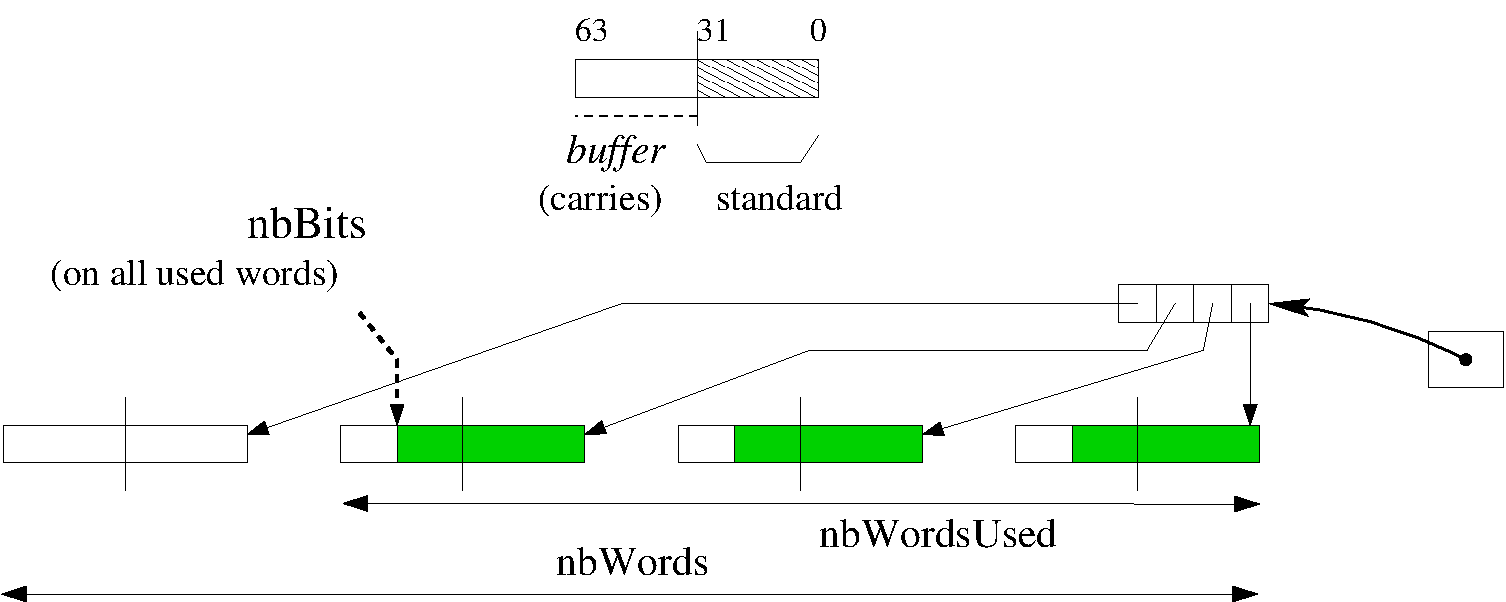
\includegraphics[scale=.5]{figures/langford/lgf_grands_entiers}
\caption{Big integer representation, 64 bits words}
\label{fig:big-integer}
\end{figure}


\paragraph{Gray sequence in memory}
The Gray sequence cannot be stored in an array because it would be too large (it would contain $2^{2n}$ byte values). This is the reason why only one part of the Gray code sequence is stored in memory and the missing terms are directly computed from the known ones using arithmetic considerations.
The size of the stored part of the Gray code sequence is chosen to be as large as possible to be contained in the processor's cache memory, the L1 cache for the GPUs threads: so the accesses are fastened and the computation of the Gray code is optimized.
For an efficient use of the E5-2650 v2 ROMEO's CPUs, which disposes of 20 MB of level-3 cache, the CPU Gray code sequence is developed recursively up to depth 25. For the K20Xm ROMEO's GPUs, which dispose of 8 KB of constant memory, the sequence is developed up to depth 15. The rest of the memory is used for the computation itself. 
%As the Gray sequence is not entirely stored in memory, 
%As we show, all the gray sequence is not in memory, in order to compute the next value when the array is exceeded a modulus method is used for recompute the next value.

\paragraph{Tasks generation and computation}
\label{sec:tasks}

In order to perform the computation of the polynomial, two variables can be set among the $2n$ available. For the tasks generation we choose a number $p$ of variables to generate $2^p$ tasks by developing the evaluation tree to depth $p$.\\
 
 
The tasks are spread over the cluster, either synchronously or asynchronously.

\textbf{Synchronous computation -}
A first experiment was carried out with an MPI distribution of the tasks of the previous model. 
Each MPI process finds its tasks list based on its process \textit{id}; then converting each task number into binary gives the task's initialization. 
The processes work independently; finally the root process ($id=0$) gathers all the computed numbers of solutions and sums them.

\textbf{Asynchronous computation -}
\label{section:asynchronous}
In this case the tasks can be computed independently. 
As with the synchronous computation, the tasks' initializations are retrieved from their number. 
Each machine can get a task,  compute it, and then store its result; then when all the tasks have been computed, the partial sums are added together and the total result is provided. 

%In this case if a task is cancel due to machine error or another problem, it can be restart without compromising the end of execution.

%\subsubsection{Efficient computation}
%The computation of any task can be summarized in the four following steps:
%\begin{itemize}
%\item First it is necessary to initialize the task: with depth level $p$, $X_1=X_2=1$ and the next $p$ variables are assigned to $1$ or $-1$ depending on the task's id. The following ones are set to $1$ for example.
%\item Secondly it is necessary to set the value of each $S_i$ with the sum of $X_kX_{k + i + 1}$.
%\item Then CPU and GPU, concurrently working, go through all of the Gray sequence on the remaining $2n-p-2$ variables, by updating the $S_i$ and sum their product at each step.
%\item Finally the CPU cores computed results are summed over a shared variable; the GPU sub-tasks results are copied back and then summed with the global result.
%\end{itemize}

\subsubsection{Experimental settings}
This part presents the experimental context and methodology, and the way the experiments were carried out.
This study has similar goals as for the Miller's resolution experiments.

\paragraph{Experimental methodology}
We present here the way the experimental settings were chosen.
Firstly we define the tasks distribution, secondly we set the number of threads per GPU block; finally, we set the CPU/GPU distribution.


\textbf{Tasks distribution depth -}
This value being set it is important to get a high number of blocks to maintain sufficient GPU load.
Thus we have to determine the best number of tasks for the distribution. As presented in part \ref{sec:tasks} the number $p$ of bits determines $2^p$ tasks. On the one hand, too many tasks are a limitation for the GPU that cannot store all the tasks in its 6GB memory. On the other hand, not enough tasks means longer tasks and too few blocks to fill the GPU grid. Fig.~\ref{fig:graphe_prof} shows that for the $L(2,23)$ instance the best task number is with generation depth 28.


\textbf{Number of threads per block -}
In order to take advantage of the GPU computation power, we have to determine the threads/block distribution. Inspired by our experiments with Miller's algorithm we know that the best value may appear at lower occupancy. We perform tests on a given tasks set varying the threads/block number and grid size associated. 
Fig.~\ref{fig:graphe_threads} presents the tests performed on the $n=20$ problem: the best distribution is around $128$ threads per block. 
\begin{figure}[htbp]
\centering 
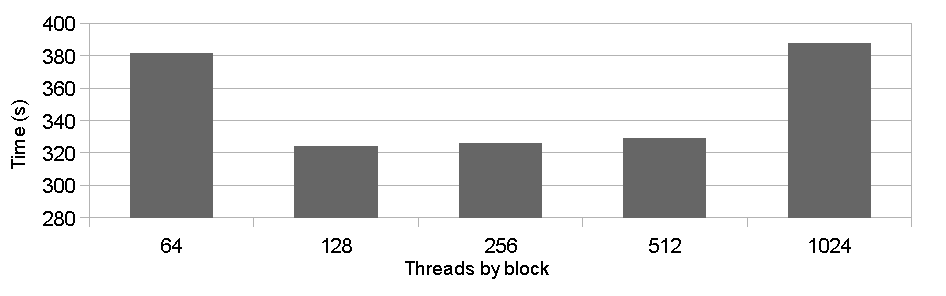
\includegraphics[scale=.55]{figures/langford/graphe_threads}
\caption{$L(2,20)$, number of threads per block}
\label{fig:graphe_threads}
\end{figure}

\begin{figure}[htb]
\begin{minipage}[b]{0.5\linewidth}

\centering 
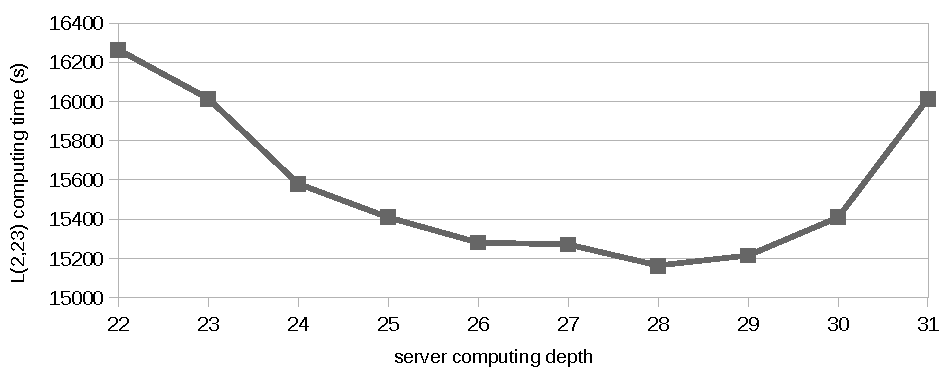
\includegraphics[scale=.5]{figures/langford/graphe_prof}
\caption{Influence on server generation depth}
\label{fig:graphe_prof}

\end{minipage}
\begin{minipage}[b]{0.5\linewidth}

\centering
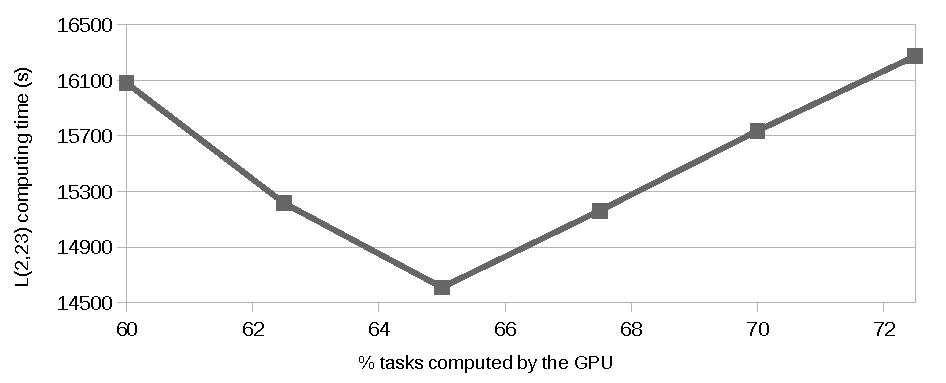
\includegraphics[scale=.5]{figures/langford/graphe_cpu_gpu}
\caption{Influence of tasks repartition}
\label{fig:graphe_rep}

\end{minipage}
\end{figure}

\paragraph{CPU vs GPU distribution -}
The GPU and CPU computation algorithm will approximately be the same. 
In order to take advantage of all the computational power of both components we have to balance tasks between CPU and GPU. 
We performed tests by changing the CPU/GPU distribution based on simulations on a chosen set of tasks.  
Fig.~\ref{fig:graphe_rep} shows that the best distribution is obtained when the GPU handles 65\% of the tasks. 
This optimal load repartition directly results from the intrinsics computational power of each component; this repartition should be adapted if using a more powerful GPU like Tesla K40 or K80.

\paragraph{Computing context}

As presented in part~\ref{sec:context}, we used the ROMEO supercomputer to perform our tests and computations.
%We use the same supercomputer to perform that computation that we use for the Miller method (section \ref{sec:context}), the ROMEO cluster which use Slurm as node reservation software.
On this supercomputer SLURM\cite{slurm} is used as a reservation and job queue manager.
This software allows two reservation modes: a static one-job limited reservation or the opportunity to dynamically submit several jobs in a Best-Effort manner.

\textbf{Static distribution -}
In this case we used the synchronous distribution presented in \ref{section:asynchronous}. 
We submited a reservation with the number of MPI processes and the number of cores per process.
This method is useful to get the results quickly if we can get at once a large amount of computation resources. It was used to perform the computation of small problems, and even for $L(2,23)$ and $L(2,24)$.\\
As an issue, it has to be noted that it is difficult to quickly obtain a very large reservation on such a shared cluster, since many projects are currently running. 

\textbf{Best effort -}
SLURM allows to submit tasks in the specific Best-Effort queue, which does not count in the user \textit{fair-share}. In this queue, if a node is free and nobody is using it, the reservation is set for a job in the best effort queue for a minimum time reservation. 
If another user asks for a reservation and requests this node, the best effort job is killed (with, for example, a SIGTERM signal). This method, based on asynchronous computation, enables a maximal use of the computational resources without blocking for a long time the entire cluster.
%This global computation process is fault-tolerant since no result is provided for aborted tasks, that are computed again.

For $L(2,27)$ and even more for $L(2,28)$ the total time required is too important to use the whole machine off a challenge period, thus we chose to compute in a Best-Effort manner.
In order to fit with this submission method we chose a reasonable time-per-task, sufficient to optimize the treatments with low loading overhead, but not too long so that killed tasks are not too penalizing for the global computation time. We empirically chose to run 15-20 minute tasks and thus we considered $p=15$ for $n=27$ and $p=17$ for $n=28$. 

The best effort based algorithm is presented on Fig.~\ref{fig:graphe_besteffort}.
The task handler maintains a maximum of 256 tasks in the queue; in addition the entire process is designed to be fault-tolerant since killed tasks have to be launched again.
When finished, the tasks generate an ouput containing the number of solutions and computation time, that is stored as a file or database entry. 
At the end the outputs of the different tasks are merged and the global result can be provided.  

\begin{figure}[htbp]
\centering
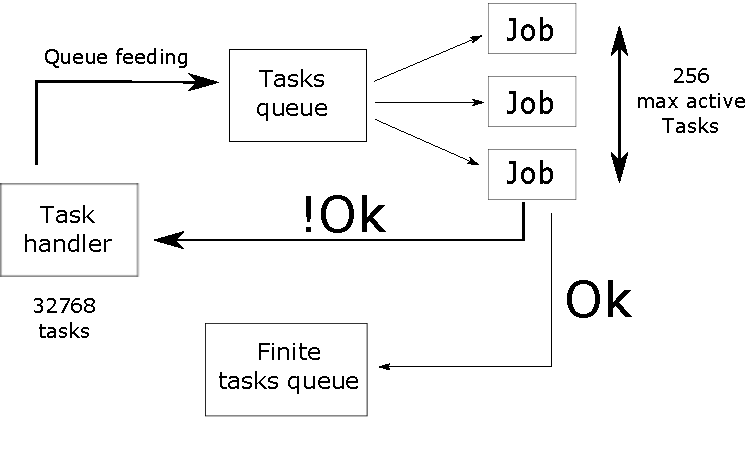
\includegraphics[scale=.6]{figures/langford/best_effort}
\caption{Best-effort distribution}
\label{fig:graphe_besteffort}
\end{figure}

%\begin{algorithm}[htbp]
%\caption{Server distribution}
%\begin{algorithmic} 
%\STATE \textbf{Variables :}
%\STATE $TQ$: tasks queue, task = integer
%\STATE $FQ$: finished tasks queue, task = integer
%\STATE $BEQ$: number of elements in the Best-Effort queue
%\STATE $N$: number of tasks
%\STATE $result$: final result
%\STATE $nbMachines$: Best-Effort queue jobs limitation
%\STATE 
%\STATE \textbf{Begin}
%\STATE $TQ\leftarrow$generate\_tasks($N$)
%\WHILE{$\#FQ \neq N$}
%\IF{$BEQ < nbMachines$}
%\STATE Start($TQ.next$)
%\ENDIF
%\ENDWHILE
%\STATE $result\leftarrow$sum($FQ$)
%\STATE \textbf{End}
%\end{algorithmic}
%\label{algo:server}
%\end{algorithm}
%
%\begin{algorithm}[htbp]
%\caption{Client task handling}
%\begin{algorithmic}
%\STATE \textbf{Variables :}
%\STATE $TQ$: tasks queue, task = integer
%\STATE $FQ$: finished tasks queue, task = integer
%\STATE $n$: number of this task
%\STATE 
%\STATE \textbf{Signal handler :}
%\IF{$SIGKILL$}
%\STATE put $n$ in the $TQ$
%\ENDIF
%\STATE 
%\STATE \textbf{Begin}
%\STATE $solution\leftarrow$compute($N$)
%\IF{$Error$}
%\STATE put $n$ in $TQ$
%\ELSE
%\STATE put $solution$ in $FQ$
%\ENDIF
%\STATE \textbf{End}
%\end{algorithmic}
%\label{algo:client}
%\end{algorithm}



\subsubsection{Results}
After these optimizations and implementation tuning steps, we conducted tests on the ROMEO supercomputer using best-effort queue to solve $L(2,27)$ and $L(2,28)$. 
We started the experiment after an update of the supercomputer, that implied a cluster shutdown. 
Then the machine was restarted and was about 50\% idle for the duration of our challenge. 
The computation lasted less than 2 days for $L(2,27)$ and 23 days for $L(2,28)$. 
The following describes performances considerations.

\textbf{Computing effort -} 
For $L(2,27)$, the effective computation time of the 32,768 tasks was about 30 million seconds (345.4 days), and 165,000" elapsed time (1.9 days); the average time of the tasks was 911", with a standard deviation of 20\%.
For the $L(2,28)$ 131,072 tasks the total computation time was about 1365 days (117 million seconds), as 23 day elapsed time; the tasks lasted 1321" on average with a 12\% standard deviation.

\textbf{Best-effort overhead -} 
With $L(2,27)$ we used a specific database to maintain information concerning the tasks: 617 tasks were aborted [by regular user jobs] before finishing (1.9\%), with an average computing time of 766" (43\% of the maximum requested time for a task). This consumed 472873", which overhead represents 1.6\% of the effective computing effort.

\textbf{Cluster occupancy -}
Fig.~\ref{fig:graphe_15minutes_27} presents the tasks resolution over the two computation days for $L(2,27)$.
The experiment elapse time was 164700" (1.9 days). Compared to the effective computation time, we used an average of 181.2 machines (CPU-GPU couples): this represents 69.7\% of the entire cluster.
 
Fig. \ref{fig:graphe_15minutes_28} presents the tasks resolution flow during the 23 days computation for $L(2,28)$. We used about 99 machines, which represents 38\% of the 230 available nodes.

\begin{figure}[htb]
\begin{minipage}[b]{0.5\linewidth}
\centering
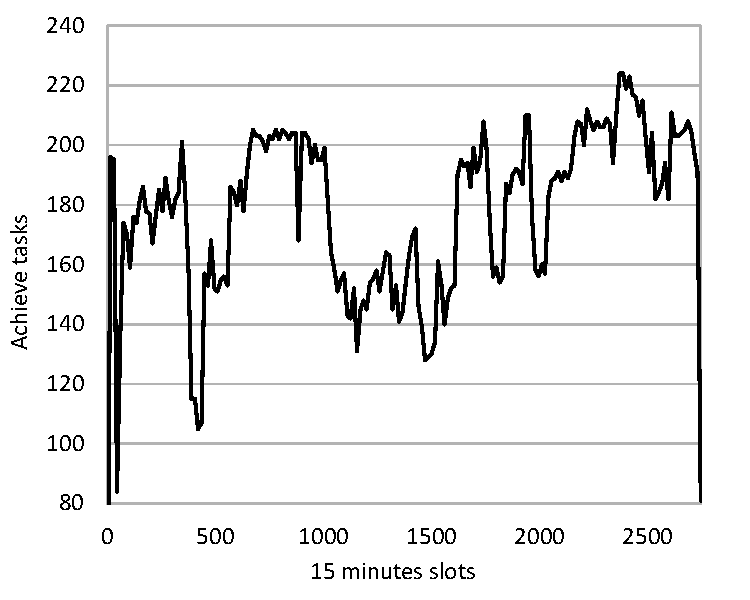
\includegraphics[scale=.6]{figures/langford/graphe_15minutes_petit}
\caption{$L(2,27)$ tasks grouped by 15" slots}
\label{fig:graphe_15minutes_27}
\end{minipage}
\begin{minipage}[b]{0.5\linewidth}
\centering
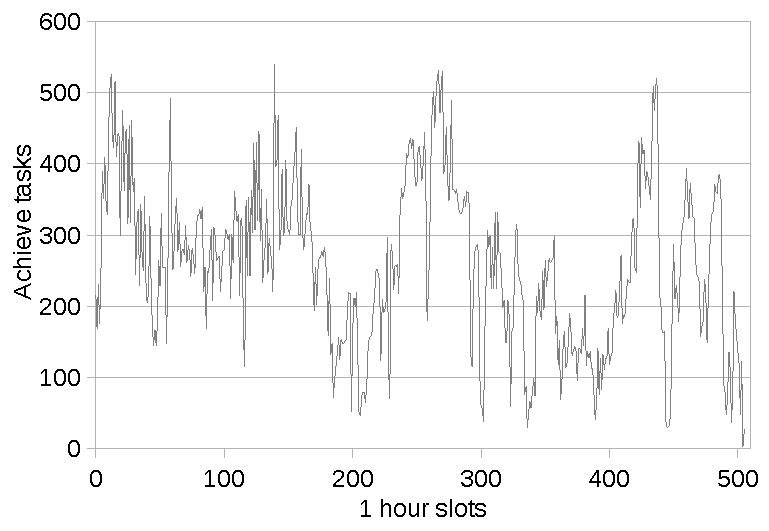
\includegraphics[scale=.6]{figures/langford/graphe_15minutes_petit_28}
\caption{$L(2,28)$ tasks grouped by 1 hour slots}
\label{fig:graphe_15minutes_28}
\end{minipage}
\end{figure}

For $L(2,27)$, these results confirm that the computation took great advantage of the low occupancy of the cluster during the experiment. 
This allowed us to obtain a weak best-effort overhead, and an important cluster occupancy. 
Unfortunately for $L(2,28)$ on such a long period we got a lower part of the supercomputer dedicated to our computational project.
Thus we are confident in good perspectives for the $L(2,31)$ instance if computed on an even larger cluster or several distributed clusters. 

\subsection{Conclusion}

This paper presents two methods to solve the Langford pairing problem on multiGPU clusters. 
In its first part the Miller's algorithm is presented. 
Then to break the problem limitations we show optimizations and implementation of Godfrey's algorithm.

\textbf{CSP resolution method -}
As any combinatorial problem can be represented as a CSP, the Miller algorithm can be seen as general resolution scheme based on the backtrack tree browsing. 
A three-level tasks generation allows to fit the multiGPU architecture. 
MPI or Best-Effort are used to spread tasks over the cluster, OpenMP for the CPU cores distribution and then CUDA to take advantage of the GPU computation power.
We were able to compute $L(2,20)$ with this regularized method and to get an even better time with the basic backtrack. 
This proves the proposed approach and also exhibits that the GPU scheduler is very efficient at managing highly divergent threads.

\textbf{MultiGPU clusters and best-effort -}
In addition and with the aim to beat the Langford limit we present a new implementation of the Godfrey method using GPUs as accelerators. In order to use the supercomputer ROMEO, which is shared by a large scientific community, we have implemented a distribution that does not affect the machine load, using a best-effort queue. The computation is fault-tolerant and totally asynchronous.

\textbf{Langford problem results -}
This study enabled us to compute $L(2,27)$ and $(L2,28)$ in respectively less than 2 days and 23 days on the University of Reims ROMEO supercomputer. The total number of solutions is: 

\hspace{3cm} L(2,27) = 111,683,611,098,764,903,232

\hspace{3cm} L(2,28) = 1,607,383,260,609,382,393,152

\textbf{Perspectives -}
This study shows the benefit of using GPUs as accelerators for combinatorial problems. 
In Miller's algorithm they handle 80\% of the computation effort and 65\% in Godfrey's.\\
As a near-term prospect, we want to scale and show that it is possible to use the order of 1000 or more GPUs for pure combinatorial problems.\\
The next step of this work is to generalize the method to optimization problems. This adds an order of complexity since shared information has to be maintained over a multiGPU cluster. 

 




\chapter{Complex systems as a benchmark} 



\section{Introduction}
The most commonly used search algorithms for graphs are Breadth First Search (BFS) and Depth First Search (DFS).
Many graph analysis methods, such as the finding of shortest path for unweighted graphs and centrality, are based on BFS. 

As it is a standard approach method in graph theory, its implementation and optimization require extensive work. 
This algorithm can be seen as frontier expansion and exploration. 
At each step the frontier is expanded with the unvisited neighbors.  
The sequential and basic algorithm is well known and is presented on Algorithm~\ref{alg:bfs_squential}.
\begin{algorithm}
\caption{Sequential BFS}\label{alg:bfs_squential}
\begin{algorithmic}[1]
\Function{compute\_BFS}{$G=(V,E)$:~graph representation, $v_s$:~source vertex, $In$:~current level input, $Out$:~current level output, $Vis$: already visited vertices}
\State $In \gets \{v_s\}$;
\State $Vis \gets \{v_s\}$;
\State $P(v) \gets \perp \forall v \in V$;
\While{$In \neq \emptyset$}
	\State $Out \gets \emptyset$
	\For{$u \in In$}
		\For{$v | (u,v) \in E$}
			\If{$v \notin Vis$}
				\State $Out \leftarrow Out \cup \{v\}$;
				\State $Vis \gets Vis \cup \{v\}$;
				\State $P(v) \leftarrow u$;
			\EndIf
		\EndFor
	\EndFor
	\State $In \gets Out$
\EndWhile
\EndFunction
\end{algorithmic}
\end{algorithm}

This algorithm is very famous thanks to its use in many applications but also thanks to the world supercomputer ranking called Graph500\footnote{\url{http://www.graph500.org}}.
This benchmark is designed to measure the performance on very irregular problems like BFS on a large scale randomized generated graph. 
The first Graph500 list was released in November 2010.
The last list, issued in November 2015, is composed of 201 machines ranked using a specific metric: Traversed Edges Per Second, denoted as TEPS. 
The aim is to perform a succession of 64 BFS on a large scale graph in the fastest possible way.
Then the ratio of edges traversed per the time of computation is used to rank the machines.

This benchmark is more representative of communication and memory accesses than computation itself. 
Other benchmarks can be used to rank computational power such as LINPACK for the TOP500 list.
Indeed the best supercomputers (K-Computer, Sequoia, Mira, ...) on the ladder have a very specific communication topology and sufficient memory, and are large enough to quickly visit all the nodes of the graph. 

In this study we focus on GPU optimization. 
There are many CPU algorithms available, which are listed on the Graph500 website. 
In order to rank the ROMEO supercomputer we had to create a dedicated version of the Graph500 benchmark in order to fit the supercomputer architecture. 
As this supercomputer is accelerated by GPUs, three successive approaches had to be applied:  first create an optimized CPU algorithm; second provide a GPU specific version and third take advantage of both CPU and GPU computation power. 

This paper is organized as follows.
The first section performs a survey of graph representation and analysis; it also describes some specific implementations.
The second section  describes the Graph500 protocol and focuses on the Kronecker graph generation method and the BFS validation.
The third section presents the chosen methods to implement graph representation and work distribution over the supercomputer nodes. It particularly focuses on the interest of a hybrid CSR and CSC representation.
We concude by examining the results for different graph scales and load distributions.

\subsection{Related work}
The most efficient algorithm to compute BFS traversal is used and detailed in \cite{6468459}. 
It uses a 2D partition of the graph which will be detailed later. 
This algorithm is used on the BlueGene/P and BlueGene/Q architectures but can be easily adapted to any parallel cluster.


We use another key study in order to build our Graph500 CPU/GPU implementation. 
This paper \cite{merrill2015high} proposes various effective methods on GPU for BFS. 
Merrill \& al. explaine and teste a few efficient methods to optimize memory access and work sharing between threads on a large set of graphs. 
It focuses on Kronecker graphs in particular. 
First they propose several methods for neighbor-gathering with a serial code versus a warp-based and a CTA-based approach. 
They also use hybridization of these methods to reach the performance level. 
In a second part they describe the way to perform label-lookup, to check if a vertex is already visited or not. 
They propose to use a bitmap representation of the graph with texture memory on the GPU for fast random accesses. 
In the last phase, they propose methods to suppress duplicated vertices generated during the neighbor exploration phase. 
Then based on these operations they propose \textit{expand-contract}, \textit{contract-expand}, \textit{two-phase} and finally \textit{hybrid} algorithms to adapt the method with all the studied graph classes.
The last part they propose a multi-GPU implementation.
They use a 1D partition of the graph and each GPU works on its subset of vertices and edges. 

In \cite{fu2014parallel}, a first work is proposed to implement a multi-GPU cluster version of the Graph500 benchmark. 
The scheme used in their approach is quite similar to the one in our study but with a more powerful communication network, namely FDR InfiniBand. 

In our work we focus on the GPUDirect usage on the ROMEO supercomputer. 

\subsection{Environment}
As previously mentioned, a CPU implementation is available on the official Graph500 website. 
A large range of software technology is covered with MPI, OpenMP, etc. 
All these versions use the same generator and the same validation pattern which is described in this part below. 

The Graph500 benchmark is based on the following stages:
\begin{itemize}
	\item \textit{Graph generation.} The first step is to generate the Kronecker graph and mix the edges and vertices. 
	The graph size is chosen by the user (represented as a based-2 number of vertices). The $EDGEFACTOR$, average ratio of edges by vertex, is always $16$. 
	Self-loop and multiple edges are possible with Kronecker graphs.
	Then 64 vertices for the BFS are randomly chosen. 
	The only rule is that a chosen vertex must have at least one link with another vertex in the graph. \textit{This stage is not timed};
	\item \textit{Structure generation.} The specific code part begins here. 
	Based on the edge list and its structure the user is free to distribute the graph over the machines. 
	In a following section we describe our choices for the graph representation. \textit{This stage is timed};
	\item \textit{BFS iterations.} This is the key part of the ranking. Based on the graph representation, the user implements a specific optimized BFS. Starting with a root vertex the aim is to build the correct BFS tree (up to a race condition at every level), storing the result in a predecessor list for each vertex;
	\item \textit{BFS verification.} The user-computed BFS is validated. The number of traversed edges is determined during this stage.  
\end{itemize}

The process is fairly simple and sources can be found at \url{http://www.graph500.org}.
The real problem is to find an optimized way to use parallelism at several levels: node distribution, CPU and GPU distribution and then massive parallelism on accelerators.



\subsubsection{Generator}

The \textit{Kronecker graphs}, based on Kronecker products, represent a specific graph class
imposed by the Graph500 benchmark. 
These graphs represent realistic networks and are very useful in our case due to their irregular aspect~\cite{leskovec2010kronecker}. 
The main generation method uses the Kronecker matrix product. 
Based on an initiator adjacency matrix $K_1$, we can generate a Kronecker graph of order $K_1^{[k]}$ by multiplying $K_1$ by itself $k$ times. 
The Graph500 generator uses Stochastic Kronecker graphs, avoiding large scale matrix multiplying, to generate an edge list which is utterly mixed (vertex number and edge position) to avoid locality. 

\begin{figure}[!t]
	\centering
	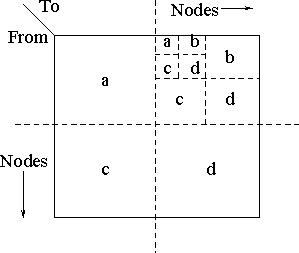
\includegraphics[scale=.9]{figures/graph500/rmat_generation}
	\caption{Kronecker generation scheme based on edge probability}
	\label{fig:kron_gen_scheme}
\end{figure}

As presented on Fig~\ref{fig:kron_gen_scheme}, the generation is based on edge presence probability on a part of the adjacency matrix. 
For the Graph500 the probabilities are $a = 0.57$, $b = c = 0.19$ and $d = 0.05$.
The generator handle can be stored in a file or directly split in the RAM memory of each process. 
The first option is not very efficient and imposes a lot of I/O for the generation and verification stage but can be very useful for large scale problems.
The second option is faster but uses a part of the RAM thus less ressources are available for the current BFS execution.


\subsubsection{Validation}
The validation stage is completed after the end of each BFS. 
The aim is to check if the tree is valid and if the edges are in the original graph.
 This is why we must keep a copy of the original graph in memory, file or RAM. 
This validation is based on the following stages, presented on the official Graph500 website.
First, the BFS tree is a tree and does not contain cycles.
Second, each tree edge connects vertices whose BFS levels differ by exactly one.
Third, every edge in the input list has vertices with levels that differ by at most one or that both are not in the BFS tree.
Finally, he BFS tree spans an entire connected component's vertices, and
a node and its parent are joined by an edge of the original graph.

In order to meet the Graph500 requirements we use the proposed verification function provided in the official code.

\subsection{BFS traversal}
In this section we present the actual algorithm we used to perform the BFS on a multi-GPU cluster. 
In a first part we introduce the data structure; then we present the algorithm and the optimizations used.

\subsubsection{Data structure}
We performed tests of several data structures.
In a first work we tried to work with bitmap. Indeed the regularity of computation can fit very well with the GPU architecture. But this representation imposes a significant limitation on the graph size. 
This representation is used on the BlueGene/Q architecture. 
Indeed they have some specific hardware bit-wise operations implemented in their processors and have a large amount of memory, allowing them to perform very large scale graph analysis. 

In a second time we used common graph representations, Compressed Sparse Row (CSR) and Compressed Sparse Column (CSC) representation, which fit very well with sparse graphs such as the Graph500 ones.
The following example illustrates the CSR representation:
$$M = \begin{pmatrix}
0 & 1 & 1 & 0 \\ 
1 & 0 & 1 & 0 \\ 
1 & 1 & 0 & 1 \\ 
0 & 0 & 1 & 0
\end{pmatrix} $$

$$R = \{0,2,4,7,8\}$$
$$C= \{1,2,0,2,0,1,3,2\}$$

The M adjacency matrix represents the graph. $R$ vector contains the cumulative number of neighbors for each vertex, of size $(\#vertices +1)$. $C$, of size $(\#edges)$, is, for each index of $R$, the edges of a vertex.
This representation is very compact and very efficient to work with sparse graphs. 

\subsubsection{General algorithm}

When looking at the latest Graph500 list we see that the best machines are the BlueGene ones. 
We count about 26 BlueGene/Q and BlueGene/P machines in the first 50  machines.
This is due to a quite specific version of the BFS algorithm proposed in \cite{6468459}. 
It proposes a very specific 2D distribution for parallelism and massive use of the 5D torus interconnect. 

In the BFS algorithm, like other graph algorithms, parallelism can take several shapes. 
We can split the vertices into partitions using 1D partition. 
Each thread/machine can then work on a subset of vertices. 
The main issue with this method is that the partitions are not equal since the number of edges per vertex can be very different; 
moreover in graphs like Kronecker ones where some vertices have a very high degree compared to other ones.
Thus we are confronted with a major load balancing problem. 

In \cite{6468459} they propose a new vision of graph traversal, here BFS, on distributed-memory machines. 
Instead of using standard 1D distribution their BFS is based on a 2D distribution. 
The adjacency matrix is split into blocks of same number of vertices.
If we consider $l\times l$ blocks $A_{i,j}$ we can split the matrix as follows:

\[ M = \left[ \begin{array}{cccc}
A_{0,0} & A_{0,1} & \cdots & A_{0,l-1} \\
A_{1,0} & A_{1,1} & \cdots & A_{1,l-1} \\
\vdots  & \vdots  & \ddots & \vdots    \\
A_{l-1,0} & A_{l-1,1}  & \cdots & A_{l-1,l-1} \end{array} \right] \] 

Each bloc $A_{x,y}$ is a subset of edges. 
We notice that blocks $A_{0,l-1}$ and $A_{l-1,0}$ have the same edges but in a reverse direction for undirected graphs. 
Based on this distribution they use \textit{virtual processors}, which are either machines or nodes, each associated with a block.
This has several advantages.
First we reduce the load balancing overhead and a communication pattern can be set up. 
Indeed each column shares the same $in\_queue$ and each row will generate an $out\_queue$ in the same range. 
Thus for all the exploration stages, communications are only on line and we just need a column communication phase to exchange the queues for the next BFS iteration.  
Algorithm~\ref{alg:bfs_bluegene} presents the BlueGene/Q and BlueGene/P parallel BFS.


\begin{algorithm}
\caption{Parallel BFS on BlueGene}\label{alg:bfs_bluegene}
\begin{algorithmic}[1]
\State $Vis_{i,j} \gets In_{i,j}$
\State $P(N_{i,j},v) \gets \bot$ \textbf{for all} $v \in R_{i,j}^{1D}$
\If{$v_s \in R_{i,j}^{1D}$}
\State $P(N_{i,j},v_s) \gets v_s$
\EndIf
\While{$true$}
	\State$(Out_{i,j},Marks_{i,j} \gets $ ExploreFrontier();
	\State $done \gets \bigwedge\limits_{0 \leq k, l \leq n} (Out_{k,l} = \emptyset)$
	\If{$done$}
		\State \textbf{exit loop}
	\EndIf
	\If{$j = 0$}
		\State $prefix_{i,j} = \emptyset$
	\Else 
		\State \textbf{receive} $prefix_{i,j}$ from $N_{i,j-1}$
	\EndIf
	\State $assigned_{i,j} \gets Out_{i,j} \setminus prefix_{i,j}$
	\If{$j \neq n -1$}
		\State \textbf{send} $prefix_{i,j} \cup Out_{i,j}$ \textbf{to} $N_{i,j+1}$
	\EndIf
	\State $Out_{i,j} \gets \bigcup\limits_{0 \leq k \leq n} Out_{i,k}$
	\State WritePred()
	\State $Vis_{i,j} \gets Vis_{i,j} \cup Out_{i,j}$
	\State $In_{i,j} \gets Out_{j,i}$
\EndWhile
\end{algorithmic}
\end{algorithm}

This algorithm is based on the exploration phase, denoted by \textit{ExploreFrontier()}. It performs the exploration phase independently on all the machines.
Then several communication phases follow. 
The first two phases are performed on the same processes line. The last one is performed on a processes column. 
\begin{itemize}
	\item On line 15, an exclusive scan is performed for each process on the same line, all the $A_{i,x}$ with $i \in [0,l-1]$. 
	This operation allows us to know which vertices have been discovered in this iteration.
	\item On line  19, a broadcast of the current $out\_queue$ is sent to the processes on the same line. With this information they would be able to update the predecessor list only if they are the first parent of a vertex.
	\item On line 24, a global communication on each column is needed to prepare the next iteration. 
	The aim is to replace the previous $in\_queue$ by the newly computed $out\_queue$.
\end{itemize}

Two functions are not specified: 
\textit{ExploreFrontier()} converts the $in\_queue$ into $out\_queue$ taking account of the previously visited vertices;
\textit{WritePred()} aims to generate the BFS tree and therefore store the predecessor list. In this algorithm the predecessor distribution is still in 1D to avoid vertex duplication. 
	This part can be done using RDMA communication to update predecessor value or with traditional MPI all-to-all exchanges.
	It can be done during each iteration stage or at the end of the BFS but this requires using a part of the memory to store this data. 

This algorithm, which is the basis of many implementations, is the main structure of our distribution. 

\subsubsection{Direction optimization}

In order to get an optimized computation in terms of TEPS we decided to sacrifice a small part of the memory for storing both the CSC and CSR representations. 
Indeed during the different BFS iterations the $in\_queue$ size varies a lot and, taking this into account, it is wiser to perform exploration from \textit{top-down} or \textit{bottom-up}. 
So, as proposed in \cite{beamer2013direction}, we perform a direction-optimized BFS.

In the first case, \textit{top-down}, we start from the vertices in the $in\_queue$ and check all the neighbors verifying each time if this neighbor has ever been visited. 
Then if not, it is added to the $out\_queue$. 
When the $in\_queue$ is sparse, like for the first and latest iterations, this method is very efficient. 
In the second case, \textit{bottom-up}, we start the exploration by the not-yet-visited vertices and verify if there is a link between those vertices and the $in\_queue$ ones. 
If yes, the not-yet-visited vertex is added to the $out\_queue$. 
Fig~\ref{fig:csr_csc} presents the two approches, whith the time visiting all the edges, and the benefits of their hybridization.

%\begin{table}
%\centering
%\begin{tabular}{|c|r|r|r|}
%		\hline 
%		Iteration & Top-down & Bottom-up & Hybridization \\ 
%		\hline 
%		%\hline 
%		0 & \color{red}{27} & 22 090 111 & \color{red}{27} \\ 
%		%\hline 
%		1 & \color{red}{8 156} & 1 568 798 & \color{red}{8 156} \\ 
%		%\hline 
%		2 & 3 695 684 & \color{blue}{587 893} & \color{blue}{587 893} \\ 
%		%\hline 
%		3 & 19 565 465 & \color{blue}{12 586} & \color{blue}{12 586} \\ 
%		%\hline 
%		4 & 214 578 & \color{blue}{8 256} & \color{blue}{8 256} \\ 
%		%\hline 
%		5 & 5 865 & \color{blue}{1 201} & \color{blue}{1 201} \\ 
%		%\hline 
%		6 & \color{red}{12} & 156 & \color{red}{12} \\ 
%		\hline
%		Total & 23,489,787 & 24,269,001 & 618,131 \\
%		\hline 
%\end{tabular} 
%\caption{BFS directions}	
%\label{table:direction_optimized}
%\end{table}

\begin{figure}[!t]
	\centering
	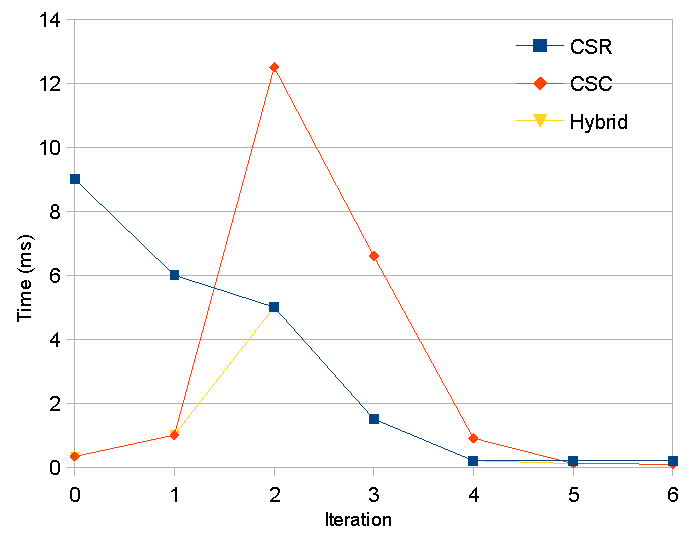
\includegraphics[width=.8\columnwidth]{figures/graph500/csr_csc_hybrid_iteration}
	\caption{CSR and CSC approach comparison. On a 6 iterations BFS, the time with the two method is compared. The hybridization just takes the best time of each method}
	\label{fig:csr_csc}
\end{figure}

\subsubsection{GPU optimization}

In algorithm \ref{alg:bfs_bluegene}, two parts are not developed. namely \textit{ExploreFrontier()} and \textit{WritePred()}. Indeed these phases are optimized using the GPU. 
Based on the Merill et al. implementation, the algorithm is optimized to use the shared memory and the texture memory of the GPU. 
For our version we decided to keep the bitmap implementation for the communications and the queues. So we have to fit the CSR and CSC implementations. 
On algorithm \ref{alg:csr} we present the CSR algorithm;
CSC is based on the same approach but starting from the $visited$ queue. 

In the CSR version each warp is attached to a 32 bit word of the $in\_queue$ bitmap. 
Then if this word is empty the whole warp is released; 
if it contains some vertices, the threads collaborate to load the entire neighbor list. 
Then they access the coalescent area in the main memory to load the neighbor list. 
A texture memory is used to accelerate the verification concerning this vertex. Indeed this memory is optimized to be randomly accessed. 
Then the vertex is added in the bitmap $out\_queue$.

\begin{algorithm}
\caption{Exploration kernel based on CSR}\label{alg:csr}
\begin{algorithmic}[1]
\State \textbf{Constants:}
\State $NWARP$: number of WARPS per block
\State 
\State \textbf{Variables:}
\State $pos\_word$: position of the word in $in\_queue$
\State $word$: value of the word in $in\_queue$
\State $lane\_id$: thread ID in the WARP
\State $warp\_id$: WARP number if this block
\State $comm[NWARP][3]$: shared memory array
\State $shared\_vertex[NWARP]$: vertex in shared memory
\State 
\State \textbf{Begin}
\If{$word = 0$}
\State free this WARP
\EndIf
\If{$word\ \& 1\ << lane\_id$}
\State $id\_sommet \gets = pos\_word*32+lane\_id$
\State $range[0] \gets C[id\_sommet]$ 
\State $range[1] \gets C[id\_sommet +1 ]$ 
\State $range[2] \gets range[1] - range[0]$ 
\EndIf
\While{$\_\_any(range[2])$}
\If{$range[2]$}
\State $comm[warp\_id][0] \gets lane\_id$
\EndIf
\If{$comm[warp\_id][0] \gets lane\_id$}
\State $comm[warp\_id][0] \gets range[0]$
\State $comm[warp\_id][0] \gets range[1]$
\State $range[2] \gets 0$
\State $share\_vertex[warp\_id] = id\_sommet$ 
\EndIf

\State $r\_gather \gets comm[warp\_id][0] + lane\_id$
\State $r\_gather\_end \gets comm[warp\_id][2] $
\While{$r\_gather < r\_gather\_end$}
	\State $voisin \gets R[r\_gather]$
	\If{$not \in tex\_visited$}
		\State Adding in $tex\_visited$
		\State AtomicOr($out\_queue$,$voisin$)
	\EndIf
	\State $r\_gather \gets r\_gather + 32$
\EndWhile
\EndWhile
\end{algorithmic}
\end{algorithm}

 
\subsubsection{Communications}

Based on the algorithm \ref{alg:bfs_bluegene} communications pattern, we first used MPI with the CPU transferring the data. But the host-device transfer time between the CPU and the GPU was too time-consuming. 
In order to accelerate the transfers between the GPUs, we used a specific GPU MPI-aware  library. This library allows direct MPI operations from the memory of one GPU to another and also implements direct GPU collective operations. 
GPUDirect can be used coupled with this library. In the last version we used this optimization with GDRCopy. 

\subsection{Results}

\subsubsection{Working environment}

All the tests were led on the ROMEO cluster available at the University of Reims Champagne-Ardenne (France).
It provides 130 nodes, each composed of 2 Ivy Bridge CPUs (8 cores), 2.6GHz and 2 Tesla K20Xm GPUs.

We used the nodes as two independent machines with one eight core CPU and one GPU attached, linked by PCIe-v3.
This allows having 260 machines for computation, each containing 32GB RAM memory and linked with QDR InfiniBand (up to 10 Gbps).
The nodes are connected with a FatTree topology. 
A K20Xm GPU has 6GB memory, 250GB/s bandwidth, 2688 CUDA cores including 896 double precision cores.

The supercomputer supports MPI with GPU Aware and GPUDirect. 
The developments were made using MVAPICH-GDR 2.2a with CUDA 7.5 \cite{nvidia2008programming} and OpenMP for the CPU implementation.

\subsubsection{CPU and GPU comparison}

\begin{figure}[!t]
\centering
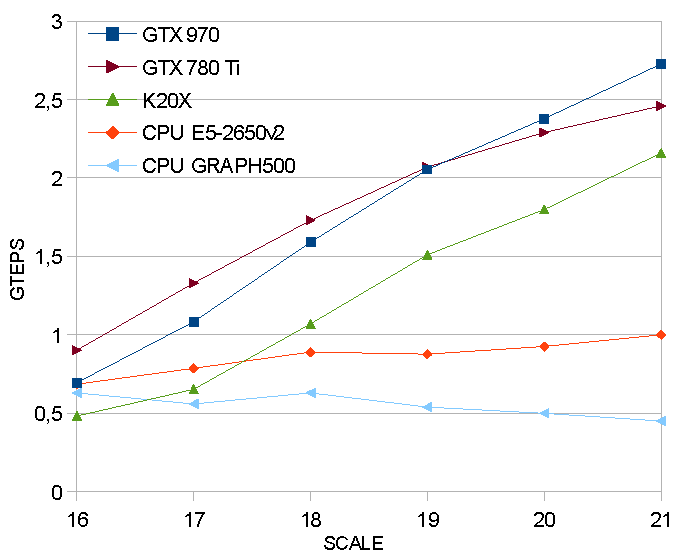
\includegraphics[width=.8\columnwidth]{figures/graph500/comparatif_GPU}
\caption[]{Single CPU and accelerators comparison. CPU Graph500 represent the best implementation proposed by the Graph500 website. }
\label{fig:single_cpu_accelerators}
\end{figure}

On Fig~\ref{fig:single_cpu_accelerators} we present the single node implementation. 
Here we compare the best CPU implementation proposed by the Graph500 benchmark with our GPU implementation. 
On our cluster we worked with K20Xm GPUs. 
The GPU result is twice times better than the CPU one. 
We also carried out tests on some "general public" GPUs like GTX980 and GTX780Ti. 
The result is better on these GPUs because they do not implement the ECC memory and do not provide double precision CUDA cores. 
Indeed all the cores can be used for the Exploration phase. 



\subsubsection{Strong and weak scaling}

On Fig~\ref{fig:bfs_strong_scaling} and Fig~\ref{fig:bfs_weak_scaling} we see the result of strong and weak scaling. 
In the strong scaling we used a $SCALE$ of $21$ for different numbers of GPUs. 
The application scales up to 16 GPUs but then the data exchanges are too penalizing;
performance for 64 GPUs is lower. 
Indeed as the problem scale does not change, the computational part is reduced compared to the communication one. 
Using 16 GPUs we were able to perform up to 4.80 GTEPS. 


For the weak scaling, the $SCALE$ evolves with the number of GPUs. 
So the computation part grows and the limitation of communications is reduced. 
On Fig~\ref{fig:bfs_weak_scaling}, the problem SCALE is presented on each point. 
With our method we were able to reach up to 12 GTEPS using this scaling. 


\subsubsection{Communications and GPUDirect}

Each node of the ROMEO supercomputer is composed of two CPU sockets and two GPUs, named GPU 0 and GPU 1.
Yet the node just has one HCA (Host Channel Adapters), linked with CPU 0 and GPU 0. 
In order to use this link GPU 1 has to pass through a Quick Path Interconnect link (QPI) between the two CPU sockets. 
This link considerably reduces the bandwidth available for node-to-node communication. 
Another problem is that the two GPUs have to share the same HCA for their communication. 


\begin{figure}[htb]
\begin{minipage}[b]{0.45\linewidth}
\centering
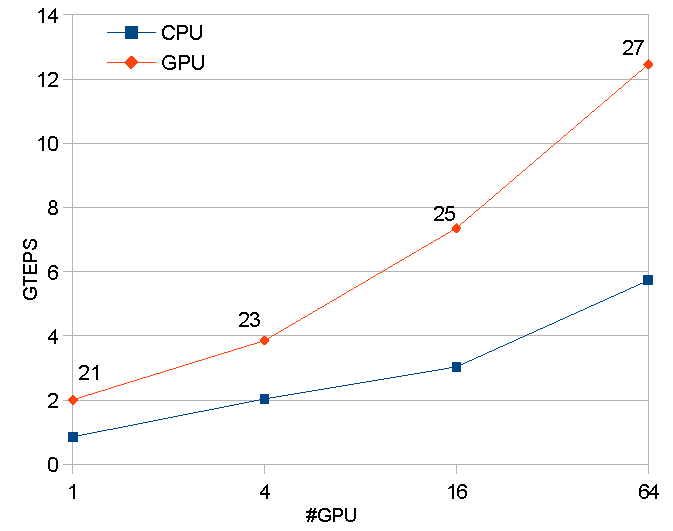
\includegraphics[width=.7\linewidth]{figures/graph500/weak_scaling}
\caption[]{CPU \textit{vs} GPU weak scaling. The number of CPUs is the same as the number of GPUs.}
\label{fig:bfs_weak_scaling}
\end{minipage}
\begin{minipage}[b]{0.45\linewidth}
\centering
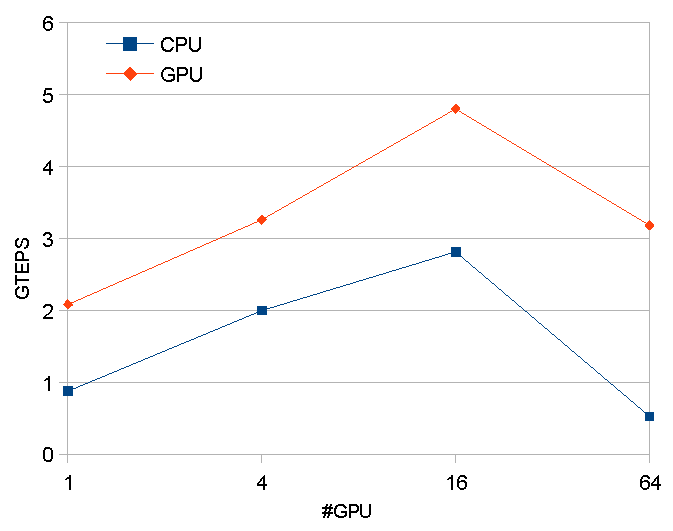
\includegraphics[width=.7\linewidth]{figures/graph500/strong_scaling}
\caption[]{CPU \textit{vs} GPU strong scaling. The $SCALE$ is showed on the GPU line. The number of CPUs is the same as the number of GPUs.}
\label{fig:bfs_strong_scaling}
\end{minipage}
\end{figure}


On Fig~\ref{fig:full_vs_gpu0}, the tests are based on the GPU-only implementation. 
First we worked with the two GPUs of the nodes. 
We were able to perform up to to $SCALE$ 29 with 12 GTEPS. 
The GPUDirect implementation does not allow the communication with a QPI link. 
So in order to compare the results, we used only the GPU 0 of each node of the supercomputer. 
Based on our algorithm implementation we need to use a number $2^{2n}$ of GPUs. 
Then the tests on Fig~\ref{fig:full_vs_gpu0} are for 256 GPUs (with GPU 0 and GPU 1) and with 64 GPUs (using just GPU 0 only). 
Thus we were able to reach a better value of GTEPS. 
As the major limitation is the communications stage, using only GPU 0 allowed us to obtain about 13.70 GTEPS on the ROMEO supercomputer. 

\begin{figure}[!t]
\centering
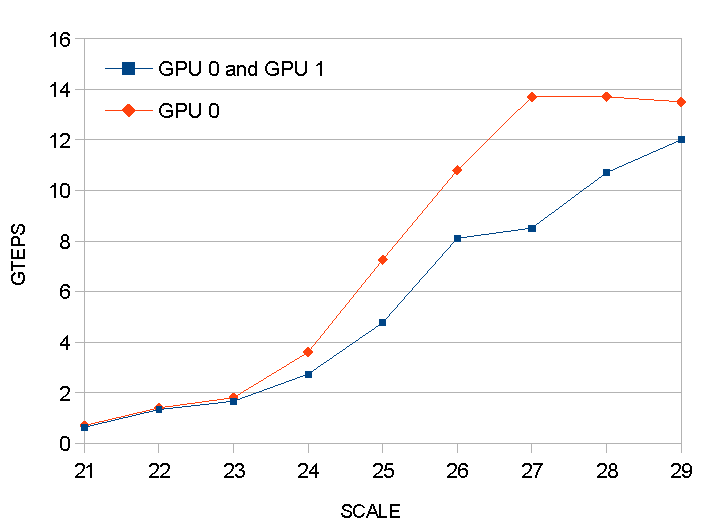
\includegraphics[width=.8\columnwidth]{figures/graph500/full_vs_gpu0}
\caption[]{Full node GPUs \textit{vs} GPU 0. The GPU 0 implementation not use the QPI link of the two CPU socket.}
\label{fig:full_vs_gpu0}
\end{figure}

\subsection{Conclusions}
In this study we present an optimized implementation of the Graph500 benchmark for the ROMEO  multi-GPU cluster. It is based on the BlueGene/Q algorithm and GPU optimization for BFS traversal by Merrill et al. 
This work highlights different key points.
First, we have chosen a hybrid memory representation of graphs using both CSR and CSC. % data representation. 
Although this representation requires more memoriy, it significantly reduces  the computation workload and allows us to achieve outstanding performance.
Second, the inter-node and intra-node communication is a critical bottleneck. 
Each compute node has two GPUs, however only one shares the same PCIe bridge with the Infiniband HCA that allows to take advantage of the GPUDirect technology.
Third, due to the low compute power needed for BFS traversal, we get better performance by fully loading GPUs.
Otherwise communication time cannot be overlapped with computation time. 
Thus to achieve the best performance we had to use only half of each node.
Finally, using all these optimizations, we achieved satisfactory results. 
Indeed, by using GPUDirect on 64 GPUs,  we are able to achieve 13,70 GTEPS. 
In this configuration CPUs are only used to synchronize GPUs kernels. 
All the communications are directly GPU to GPU using a CUDA-aware MPI library and GPUDirect.

These results will be published in the next Graph500 list. With a total of 13.70 GTEPS the ROMEO supercomputer could be ranked at the 91th position. 

Today we can identify some interesting perspectives to carry on the study. 
Communication cost is the major limitation and a better control of load distribution is needed between communication and computation in order to obtain even better performance.
Part of the solution might come from new technologies developed by Nvidia, such as the new PASCAL architecture or NVlink buses.
 
\section{Conclusion}